\documentclass[tikz,border=3.14mm]{standalone}
\usetikzlibrary{positioning}

\begin{document}
	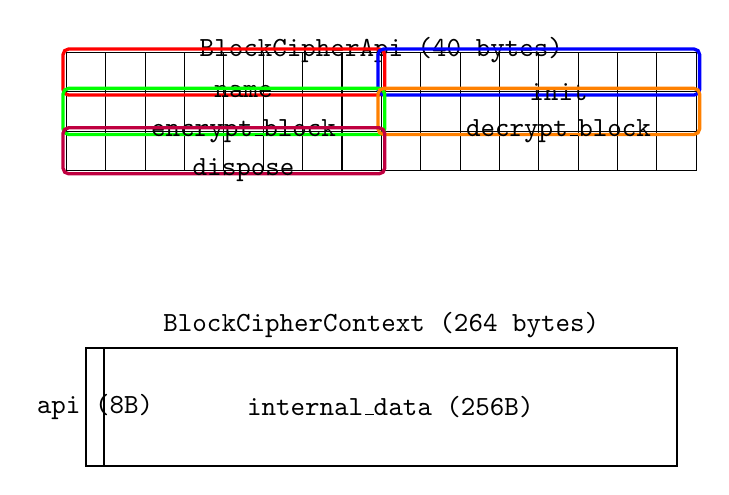
\begin{tikzpicture}[font=\ttfamily]
		
		% --- Diagram for BlockCipherApi (40 bytes) ---
		% Each cell represents 1 byte.
		% Layout:
		%   Row 0 (offsets 0x00–0x0F):
		%     - Columns 0–7:  "name" (8 bytes)
		%     - Columns 8–15: "init" (8 bytes)
		%   Row 1 (offsets 0x10–0x1F):
		%     - Columns 0–7:  "encrypt_block" (8 bytes)
		%     - Columns 8–15: "decrypt_block" (8 bytes)
		%   Row 2 (offsets 0x20–0x2F):
		%     - Columns 0–7:  "dispose" (8 bytes)
		%
		\def\cellSize{0.5} % size of each cell in cm
		
		% Draw grid: 3 rows and 16 columns
		\foreach \row in {0,1,2} {
			\foreach \col in {0,...,15} {
				\node[draw, minimum size=\cellSize cm] (AP\row\col) at (\col*\cellSize, -\row*\cellSize) {};
			}
		}
		% Title for the API layout
		\node[above] at (7.5*\cellSize, 0) {BlockCipherApi (40 bytes)};
		
		% Draw block for "name" (offsets 0x00–0x07): Row 0, columns 0 to 7.
		\draw[red, very thick, rounded corners=2pt]
		([shift={(-1pt,1pt)}]AP00.north west) rectangle ([shift={(1pt,-1pt)}]AP07.south east);
		\node at (4*\cellSize, -0.5*\cellSize) {name};
		
		% Draw block for "init" (offsets 0x08–0x0F): Row 0, columns 8 to 15.
		\draw[blue, very thick, rounded corners=2pt]
		([shift={(-1pt,1pt)}]AP08.north west) rectangle ([shift={(1pt,-1pt)}]AP015.south east);
		\node at (12*\cellSize, -0.5*\cellSize) {init};
		
		% Draw block for "encrypt_block" (offsets 0x10–0x17): Row 1, columns 0 to 7.
		\draw[green, very thick, rounded corners=2pt]
		([shift={(-1pt,1pt)}]AP10.north west) rectangle ([shift={(1pt,-1pt)}]AP17.south east);
		\node at (4*\cellSize, -1.5*\cellSize) {encrypt\_block};
		
		% Draw block for "decrypt_block" (offsets 0x18–0x1F): Row 1, columns 8 to 15.
		\draw[orange, very thick, rounded corners=2pt]
		([shift={(-1pt,1pt)}]AP18.north west) rectangle ([shift={(1pt,-1pt)}]AP115.south east);
		\node at (12*\cellSize, -1.5*\cellSize) {decrypt\_block};
		
		% Draw block for "dispose" (offsets 0x20–0x27): Row 2, columns 0 to 7.
		\draw[purple, very thick, rounded corners=2pt]
		([shift={(-1pt,1pt)}]AP20.north west) rectangle ([shift={(1pt,-1pt)}]AP27.south east);
		\node at (4*\cellSize, -2.5*\cellSize) {dispose};
		
		% --- Diagram for BlockCipherContext (264 bytes) ---
		% Layout:
		%   - Field "api": occupies the first 8 bytes (offset 0 to 7).
		%   - Field "internal_data": occupies the next 256 bytes (offset 8 to 263).
		\begin{scope}[yshift=-3.5cm] % shift down for the second diagram
			
			% Define overall width and height for visualization (arbitrary dimensions)
			\def\contextWidth{7.5}  % in cm
			\def\contextHeight{1.5} % in cm
			
			% Draw the overall rectangle for BlockCipherContext.
			\draw[thick] (0,0) rectangle (\contextWidth, -\contextHeight);
			\node[above] at (\contextWidth/2, 0) {BlockCipherContext (264 bytes)};
			
			% Compute the width corresponding to the 8-byte "api" field.
			\pgfmathsetmacro{\apiWidth}{\contextWidth * 8 / 264}
			
			% Draw vertical divider
			\draw[thick] (\apiWidth, 0) -- (\apiWidth, -\contextHeight);
			
			% Label the two regions.
			\node at (\apiWidth/2, -\contextHeight/2) {api (8B)};
			\node at ({\apiWidth + (\contextWidth - \apiWidth)/2}, -\contextHeight/2) {internal\_data (256B)};
		\end{scope}
		
	\end{tikzpicture}
\end{document}
